%!TEX root = ../slopecd.tex
\section{Theory}\label{sec:theory}
%%%%%%%%%%%%%%%%%%%%%%%%%%%%%%%%%%%%
\subsection{Directional Derivatives}%
\label{sec:directional-derivatives}
%%%%%%%%%%%%%%%%%%%%%%%%%%%%%%%%%%%%

\subsubsection{The Sorted \texorpdfstring{\(\ell_1\)}{l1}
  Norm}

\begin{theorem}
  \label{thm:sl1-directional-derivative} Let \(h_0 \in \big(0, \min_{i,j \in
    \{i \mid \beta_i \neq 0\}}\big| |\beta_i| - |\beta_j| \big|/\max_k|v_k| \big]\) and
  define \(\sigma\) to be the permutation such that
  \[
    |\beta + h_0v|_{\sigma(1)} \geq |\beta + h_0v |_{\sigma(2)}
    \geq \cdots \geq |\beta + h_0v|_{\sigma(p)}.
  \]
  The directional derivative for the sorted \(\ell_1\) norm, \(J(\beta)\), is
  \[
    D_v J(\beta) =
    \sum_i \sum_{j \in \mathcal{B}_i} \lambda_j v_{\sigma(j)}\sign(\beta_{\sigma(j)} + h_0v_{\sigma(j)})\]
  where
  \[
    \mathcal{B}_i = \{j \mid |\beta_j| = c_i\},\qquad
    c_1 > c_2 > \cdots > c_m \geq 0,
  \]
  such that \(m\) is the number of clusters.
  \jl{We need something that doesn't define clusters multiple times.}
  \mathurin{Good remark, I guess we could avoid naming the variable \(i\) since above we have \(i\) and \(j\) being both in \([p]\) while here \(i\) would in fact be in \([n_{clusters}/n_{groups}]\). \(g\) for groups, as used in group Lasso? "For a fixed \(\beta\), let \(G\) be the number of different values taken by \(\abs{\beta_j}\), i.e. the number of groups, and let \((\cB_g)_{g \in G}\) be a partition of \([p]\) such that \(\forall (j, j') \in \cB_g, \abs{\beta_j} = \abs{\beta_{j'}}\)}
  \jl{Thanks, yes that would work.
    I have tried something slightly different
    here, however, which may be enough for us.
  }

\end{theorem}
\begin{proof}
  The directional derivative for the sorted \(\ell_1\) norm and a direction
  \(v\) with \(\lVert v \rVert = 1\) is
  \begin{equation}
    \label{eq:sl1-directional-derivative}
    \begin{aligned}
      D_v J(\beta) & = \lim_{h \searrow 0} \frac{J(\beta + h v) - J(\beta)}{h}                                                                    \\
                   & = \lim_{h \searrow 0} \frac{\sum_{j=1}^p\lambda_j\big(|\beta + vh|_{\sigma(j)} - |\beta|_{(j)}\big)}{h}                      \\
                   & = \lim_{h \searrow 0}\frac{\sum_i \sum_{j \in \mathcal{B}_i} \lambda_j\big(|\beta + vh|_{\sigma(j)} - |\beta|_{(j)}\big)}{h} \\
    \end{aligned}
  \end{equation}
  Assume without loss of generality that \(c_m = 0\).
  Then
  \[
    \sum_{j \in \mathcal{B}_m}\frac{\lambda_j \big( |\beta + vh|_{\sigma(j)} - |\beta|_{(j)}\big)}{h}
    = \sum_{j \in \mathcal{B}_m} \lambda_j \sign(\beta + hv)_{\sigma(j)}v_{\sigma(j)}.
  \]
  Next, recall the construction of \(h_0\) and
  observe that \(\sign(\beta_j + hv_j) = \sign(\beta_j)\)
  and \(\sigma(j) = (j)\) for all \(j \notin \mathcal{B}_m\)
  whenever \(0 < h < h_0\).
  It follows that
  \[
    \sum_{j \in \mathcal{B}_i} \frac{\lambda_j\big(|\beta + hv|_{\sigma(j)} - |\beta|_{(j)}\big)}{h}
    = \sum_{j \in \mathcal{B}_i} \lambda_j\sign(\beta + vh)_{\sigma(j)}v_{\sigma(j)}.
  \]
  From this, we see that \eqref{eq:sl1-directional-derivative} reduces to
  \[
    \lim_{h \searrow 0} \sum_i \sum_{j \in \mathcal{B}_i} \lambda_j\sign(\beta + vh)_{\sigma(j)}v_{\sigma(j)}
    = \sum_i \sum_{j \in \mathcal{B}_i} \lambda_j\sign(\beta + vh_0)_{\sigma(j)}v_{\sigma(j)}.
  \]
\end{proof}

\begin{remark}
  Using \cref{thm:sl1-directional-derivative}, we see that
  the directional derivative for \eqref{eq:slope-problem} is
  \[
    D_v P(\beta) = v^T \big(\nabla L(\beta)\big) + D_v J(\beta).
  \]
\end{remark}

\subsection{Coordinate Updates}%
\label{sec:coordinate-updates}

Assume that we want to compute the coordinate update for the \(q\)th cluster
\(\mathcal{C}_q\) under the constraint that \(\sign(\beta) = s\).
We have
\jl{Need to redefine permutation to act on \(c\) instead.}
\[
  \begin{aligned}
    P(\beta) & = \frac{1}{2} \lVert y - X\beta\rVert_2^2 + J(\beta)                                                                                                                                                                                                                        \\
             & = \frac{1}{2} \lVert y - X_{\bar{\mathcal{C}_q}} \beta_{\bar{\mathcal{C}_q}} - z X_{\mathcal{C}_q} s_{\mathcal{C}_q} \rVert_2^2 + \sum_{k \notin {\mathcal{C}_q}} \lambda_{(k)^-}|\beta_k| + |z|\sum_{k \in {\mathcal{C}_q}} \lambda_{(k)^-}                                                                                                                            \\
             & = \splitfrac{\frac{1}{2} \left(y^Ty - 2y^T X_{\bar{\mathcal{C}_q}} \beta_{\bar{\mathcal{C}_q}} - 2 z y^T X_{\mathcal{C}_q} s_{\mathcal{C}_q} + 2 z (X_{\mathcal{C}_q} s_{\mathcal{C}_q})^T X_{\bar{\mathcal{C}_q}} \beta_{\bar{\mathcal{C}_q}} + \lVert X_{\bar{\mathcal{C}_q}} \beta_{\bar{\mathcal{C}_q}} \rVert_2^2 + z^2 \lVert X_{\mathcal{C}_q} s_{\mathcal{C}_q}\rVert_2^2 \right)}{+ \sum_{k \notin {\mathcal{C}_q}} \lambda_{(k)^-}|\beta_k| + |z|\sum_{k \in {\mathcal{C}_q}} \lambda_{(k)^-}} \\
  \end{aligned}
\]
Taking the derivative with respect to \(z\) yields
\[
  \frac{\partial}{\partial z}P(\beta) = -y^T X_{\mathcal{C}_q} s_{\mathcal{C}_q} + (X_{\bar{\mathcal{C}_q}} \beta_{\bar{\mathcal{C}_q}})^T{X_{\mathcal{C}_q} s_{\mathcal{C}_q}} + z \lVert X_{\mathcal{C}_q} s_{\mathcal{C}_q} \rVert_2^2 + \frac{\partial}{\partial z}|z|\sum_{k \in {\mathcal{C}_q}} \lambda_{(k)^-}.
\]
The optimality condition for this sub-problem is
\[
  z + \frac{(X_{\mathcal{C}_q} s_{\mathcal{C}_q})^T\left( X_{\bar{\mathcal{C}_q}}\beta_{\bar{\mathcal{C}_q}} - y \right) + \frac{\partial}{\partial z}|z|\sum_{k \in {\mathcal{C}_q}} \lambda_{(k)^-}}{s_{\mathcal{C}_q}^T X_{{\mathcal{C}_q}}^T X_{\mathcal{C}_q} s_{\mathcal{C}_q}} \in \boldsymbol{0}.
\]

\begin{figure}[htbp]
  \centering
  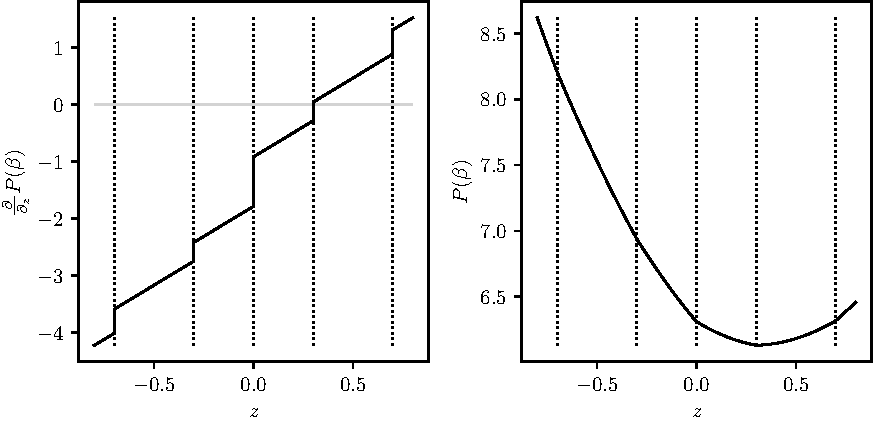
\includegraphics[]{figures/clusterupdate-grad-obj}
  \caption{%
    Objective and gradient under the constraint that we have a fixed
    cluster. The optimum is found at \(z = 0.3\).
  }
  \label{fig:cluster-grad-obj}
\end{figure}



